\documentclass[10pt]{article}
\usepackage[a4paper,margin=2cm]{geometry}
\usepackage[T1]{fontenc}
\usepackage{lmodern}
\usepackage{booktabs}
\usepackage{graphicx}
\usepackage{amsmath}
\usepackage{microtype}
\usepackage[hidelinks]{hyperref}
\usepackage{xcolor}
\usepackage{caption}
\captionsetup{font=small,labelfont=bf,skip=3pt}
\setlength{\parskip}{2pt}
\setlength{\parindent}{0pt}
\graphicspath{{../results/figures/}}

% Auto-generated by src/make_report_assets.py
\newcommand{\fullAcc}{84.8}
\newcommand{\fullFone}{84.6}
\newcommand{\fullTrainAcc}{99.7}
\newcommand{\fullGap}{14.8}
\newcommand{\fullTime}{37.1}
\newcommand{\fullParams}{1,555,781}
\newcommand{\fullEpoch}{10}
\newcommand{\headAcc}{87.0}
\newcommand{\headFone}{86.9}
\newcommand{\headTrainAcc}{99.9}
\newcommand{\headGap}{12.9}
\newcommand{\headTime}{13.8}
\newcommand{\headParams}{628,773}
\newcommand{\headEpoch}{14}
\newcommand{\lrAcc}{85.4}
\newcommand{\lrFone}{85.3}
\newcommand{\lrTrainAcc}{98.7}
\newcommand{\lrGap}{13.3}
\newcommand{\lrTime}{2.1}
\newcommand{\lrConfig}{C=0.01}
\newcommand{\svmAcc}{83.9}
\newcommand{\svmFone}{83.6}
\newcommand{\svmTime}{2.3}
\newcommand{\rfAcc}{83.0}
\newcommand{\rfFone}{82.5}
\newcommand{\rfTime}{2.2}
\newcommand{\extractTime}{2.1}
\newcommand{\worstClass}{american pit bull terrier}
\newcommand{\worstFone}{60.9}
\newcommand{\bestClass}{keeshond}
\newcommand{\bestFone}{98.0}
\newcommand{\topPairA}{american pit bull terrier}
\newcommand{\topPairB}{staffordshire bull terrier}
\newcommand{\topPairCount}{25}
\newcommand{\topPairFrac}{25.0}
\newcommand{\fullVal}{89.7}
\newcommand{\headVal}{90.1}
\newcommand{\headLrDiff}{1.6}
\newcommand{\timeRatioFH}{2.7}
\newcommand{\fullHeadDiff}{2.2}
\newcommand{\lrFullDiff}{+0.6}
\newcommand{\costRatio}{18}
\newcommand{\pFullLr}{=0.28}
\newcommand{\pFullHead}{<0.001}
\newcommand{\pHeadLr}{<0.001}
\newcommand{\sharedErrors}{357}
\newcommand{\lrErrors}{534}


\title{\vspace{-1.2cm}\textbf{Transfer Learning for Fine-Grained Pet Breed Classification}\\[2pt]
\large A comparison of full fine-tuning, classifier-head training, and frozen features}
\author{Shihab Uddin}
\date{Computer Vision --- Fall 2026}

\begin{document}
\maketitle
\vspace{-0.6cm}

\begin{abstract}
\noindent
We adapt an ImageNet-pretrained MobileNetV3-Small to the 37 breed classes of the
Oxford-IIIT Pet dataset and compare three transfer-learning strategies under one fixed
data split and evaluation protocol: full fine-tuning, training only the classifier head,
and a scikit-learn classifier on frozen penultimate features. Training only the
classifier head is both the most accurate and the cheapest neural strategy: \headAcc\%
test accuracy (macro-F1 \headFone\%) in \headTime{} minutes, significantly better than
full fine-tuning (\fullAcc\%, macro-F1 \fullFone\%, \fullTime{} minutes; exact McNemar
$p\pFullHead$). Logistic regression on the same frozen features reaches \lrAcc\%
(macro-F1 \lrFone\%) in \lrTime{} minutes, \headLrDiff{} points below the head but almost
an order of magnitude cheaper. With roughly 3k training images, freezing the backbone
regularizes training and outperforms updating all weights.
\end{abstract}

\section{Introduction}
Fine-grained visual classification requires separating categories that share an overall
shape and differ mainly in local texture, colour, and proportions. Oxford-IIIT Pet is a
compact benchmark for this setting: 37 cat and dog breeds with roughly 200 images each,
substantial variation in pose, scale, and lighting, and a non-trivial domain gap from
ImageNet. Training a deep network from scratch on such a small dataset is unlikely to
work well, so we start from ImageNet-1K weights and ask how much of the network should
be adapted.

We compare three strategies that are identical in data, preprocessing, and evaluation:
(i) updating the whole network, (ii) freezing the convolutional feature extractor and
training only the fully connected head, and (iii) using the frozen network as a feature
extractor and training a traditional classifier on its 576-dimensional penultimate
representation. Besides accuracy and macro-F1, we report trainable parameter counts and
wall-clock cost, and we analyse the confusion structure and the train/test gap.

\section{Dataset and splits}
The Oxford-IIIT Pet dataset \cite{parkhi2012cats} contains 37 breeds (12 cats, 25 dogs)
and 7,390 JPEG images. Images are annotated with breed, a head bounding box, and a
pixel-level trimap; we use only the breed labels. The dataset is distributed for
research purposes only, and the images remain subject to the terms of use of the sites
from which they were collected; we therefore do not redistribute the data. It can be
obtained from \url{https://www.robots.ox.ac.uk/~vgg/data/pets/} by extracting
\texttt{images.tar.gz} and \texttt{annotations.tar.gz}.

We use the official \texttt{trainval}/\texttt{test} partitions, which list 7,349 images
in total; all of them are present, and 41 of the 7,390 JPEG files in the archive are not
referenced by the lists and are ignored. The official
trainval partition (3,680 images) is split once into 2,944 training and 736 validation
images with an 80/20 stratified split by breed (seed 42); the 3,669-image test partition
is kept separate and is touched only for the final evaluation. Table~\ref{tab:counts}
lists the per-breed counts. The split manifests are stored as CSV files in the
repository, so every method uses exactly the same images.

\begin{table}[t]
\centering
\caption{Images per breed in each split. The official test partition is never used for
training or model selection.}
\label{tab:counts}
\scriptsize
\begin{tabular}{lrrrr@{\hskip 12pt}lrrrr}
\toprule
Breed & Train & Val & Test & Total & Breed & Train & Val & Test & Total \\
\midrule
Abyssinian & 80 & 20 & 98 & 198 & leonberger & 80 & 20 & 100 & 200 \\
american bulldog & 80 & 20 & 100 & 200 & Maine Coon & 80 & 20 & 100 & 200 \\
american pit bull terrier & 80 & 20 & 100 & 200 & miniature pinscher & 80 & 20 & 100 & 200 \\
basset hound & 80 & 20 & 100 & 200 & newfoundland & 77 & 19 & 100 & 196 \\
beagle & 80 & 20 & 100 & 200 & Persian & 80 & 20 & 100 & 200 \\
Bengal & 80 & 20 & 100 & 200 & pomeranian & 80 & 20 & 100 & 200 \\
Birman & 80 & 20 & 100 & 200 & pug & 80 & 20 & 100 & 200 \\
Bombay & 77 & 19 & 88 & 184 & Ragdoll & 80 & 20 & 100 & 200 \\
boxer & 80 & 20 & 99 & 199 & Russian Blue & 80 & 20 & 100 & 200 \\
British Shorthair & 80 & 20 & 100 & 200 & saint bernard & 80 & 20 & 100 & 200 \\
chihuahua & 80 & 20 & 100 & 200 & samoyed & 80 & 20 & 100 & 200 \\
Egyptian Mau & 74 & 19 & 97 & 190 & scottish terrier & 80 & 20 & 99 & 199 \\
english cocker spaniel & 77 & 19 & 100 & 196 & shiba inu & 80 & 20 & 100 & 200 \\
english setter & 80 & 20 & 100 & 200 & Siamese & 79 & 20 & 100 & 199 \\
german shorthaired & 80 & 20 & 100 & 200 & Sphynx & 80 & 20 & 100 & 200 \\
great pyrenees & 80 & 20 & 100 & 200 & staffordshire bull terrier & 80 & 20 & 89 & 189 \\
havanese & 80 & 20 & 100 & 200 & wheaten terrier & 80 & 20 & 100 & 200 \\
japanese chin & 80 & 20 & 100 & 200 & yorkshire terrier & 80 & 20 & 100 & 200 \\
keeshond & 80 & 20 & 99 & 199 & & & & &  \\
\midrule
Total & 2944 & 736 & 3669 & 7349 & & & & & \\
\bottomrule
\end{tabular}
\end{table}

\paragraph{Preprocessing and augmentation.}
All images are resized with the transformation associated with the pre-trained weights.
Training uses \texttt{RandomResizedCrop(224, scale=(0.65,1))}, a random horizontal flip,
and mild colour jitter (brightness/contrast 0.25, saturation 0.2, hue 0.03). Validation
and test images are resized so that the shorter side is 256 and centre-cropped to
$224\times224$. All splits use ImageNet normalization
($\mu=[0.485,0.456,0.406]$, $\sigma=[0.229,0.224,0.225]$). Augmentation is applied to
the training set only. The dataset is almost balanced (79--80 training images per
breed), so no re-weighting or resampling is used; accuracy and macro-F1 are therefore
both meaningful.

\section{Methods}
\subsection{Backbone and classifier head}
All experiments use \texttt{torchvision.models.mobilenet\_v3\_small} with
\texttt{MobileNet\_V3\_Small\_Weights.DEFAULT} (ImageNet-1K) \cite{howard2019mobilenetv3},
implemented in PyTorch \cite{paszke2019pytorch}.
The original 1,000-way final layer is replaced by \texttt{Linear(1024, 37)}, giving a
network with 1,555,781 parameters in total. The classifier block is
$\text{Linear}(576,1024) \rightarrow \text{Hardswish} \rightarrow \text{Dropout}(0.2)
\rightarrow \text{Linear}(1024,37)$.

\subsection{Adaptation strategies}
\textbf{Full fine-tuning.} The whole network, including all convolutional layers, is
trained (\fullParams{} trainable parameters).

\textbf{Classifier-head training.} The feature extractor (\texttt{features} and
\texttt{avgpool}) is frozen. The only trainable layers are \texttt{classifier[0]}
($576\rightarrow1024$) and \texttt{classifier[3]} ($1024\rightarrow37$); Hardswish and
Dropout have no parameters. This gives \headParams{} trainable parameters, 40.4\% of the
full model. The frozen extractor is kept in evaluation mode throughout, so its BatchNorm
running statistics stay at their ImageNet values instead of drifting towards the pet
training set; in a pilot run that left the backbone in training mode, the statistics
drifted and validation macro-F1 fell by more than six points.

\textbf{Frozen features with a traditional classifier.} The frozen network maps each
image to the 576-dimensional output of \texttt{features} followed by global average
pooling, i.e.\ the input of \texttt{classifier[0]}. Features are extracted once for
train, validation, and test. A \texttt{StandardScaler} is fit on the training features
only and applied to all splits. We compare multinomial logistic regression, a linear SVM,
and a 500-tree random forest. For logistic regression and the SVM, the regularization
strength is chosen from $C\in\{10^{-3},10^{-2},10^{-1},1\}$ by validation macro-F1; the
random forest uses scikit-learn defaults with \texttt{sqrt} feature subsampling
\cite{pedregosa2011sklearn}. No dimensionality reduction was necessary at 576 dimensions.

\subsection{Training protocol and model selection}
Both neural models use AdamW, batch size 32, cross-entropy with label smoothing 0.1, and
a one-epoch linear warm-up followed by cosine decay. Full fine-tuning runs for 12 epochs
at $\mathrm{lr}=3\times10^{-4}$; head-only training runs for 15 epochs at
$\mathrm{lr}=10^{-3}$; weight decay is $10^{-4}$ in both cases. Training uses CPU
bfloat16 autocast. After every epoch we compute validation accuracy and macro-F1, and we
keep the checkpoint with the best validation macro-F1. The test set is never used for
early stopping, hyper-parameter selection, or threshold selection. All runs use seed 42
for Python, NumPy, and PyTorch; deterministic algorithms are requested where available.
The selected checkpoint is evaluated exactly once on the test set. Training times are
measured on the same 4-core CPU machine for all methods; the scikit-learn times include
the one-off feature extraction (\extractTime{} minutes).

\section{Results}
Table~\ref{tab:results} summarises test performance and cost. Head-only training gives
the highest test accuracy (\headAcc\%, macro-F1 \headFone\%), significantly above full
fine-tuning (\fullAcc\%; exact McNemar $p\pFullHead$) and above logistic regression on
the same frozen features (\lrAcc\%; $p\pHeadLr$). Full fine-tuning and logistic
regression are statistically indistinguishable ($p\pFullLr$), and
\sharedErrors{} of the \lrErrors{} logistic-regression errors are also full fine-tuning
errors, so the two fail on largely the same images. Among the other traditional
classifiers, the linear SVM reaches \svmAcc\% and the random forest \rfAcc\%. Validation
agrees with the test ranking for the two neural models (head \headVal\% versus full
\fullVal\%), and the paired tests, not the raw ordering, support the conclusions.

\begin{table}[t]
\centering
\caption{Test results (official test split, evaluated once). ``Train acc.'' is accuracy
on the unaugmented training set of the selected checkpoint; ``Gap'' is train minus test
accuracy in percentage points. Times for the scikit-learn rows include the shared
\extractTime-minute feature extraction, and their parameter count is the number of
classifier coefficients ($576\times37+37$); the feature extractor is fixed.}
\label{tab:results}
\footnotesize
\begin{tabular}{lrrrrrr}
\toprule
Approach & Trainable & Time & Test & Macro & Train & Gap \\
 & params & (min) & acc.\ (\%) & F1 (\%) & acc.\ (\%) & (pp) \\
\midrule
Full fine-tuning & 1,555,781 & 37.1 & 84.8 & 84.6 & 99.7 & +14.8 \\
Classifier head only & 628,773 & 13.8 & 87.0 & 86.9 & 99.9 & +12.9 \\
Logistic regression (frozen) & 21,349 & 2.1 & 85.4 & 85.3 & 98.7 & +13.3 \\
Linear SVM (frozen) & 21,349 & 2.3 & 83.9 & 83.6 & 95.7 & +11.7 \\
Random forest (frozen) & 21,349 & 2.2 & 83.0 & 82.5 & 100.0 & +17.0 \\
\bottomrule
\end{tabular}
\end{table}

\begin{figure}[t]
\centering
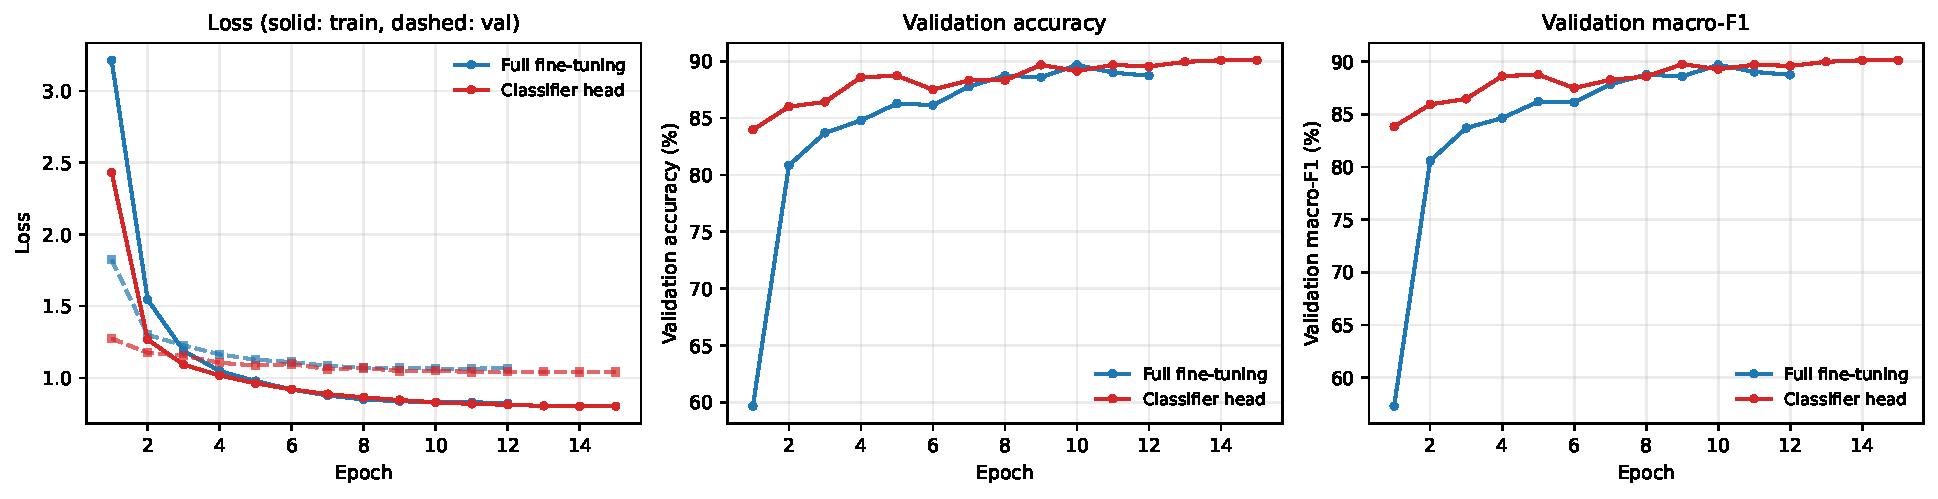
\includegraphics[width=\textwidth]{training_curves.pdf}
\caption{Validation behaviour of the two neural strategies. Full fine-tuning improves
steadily; head-only training converges faster and ends at a higher validation macro-F1.}
\label{fig:curves}
\end{figure}

\begin{figure}[t]
\centering
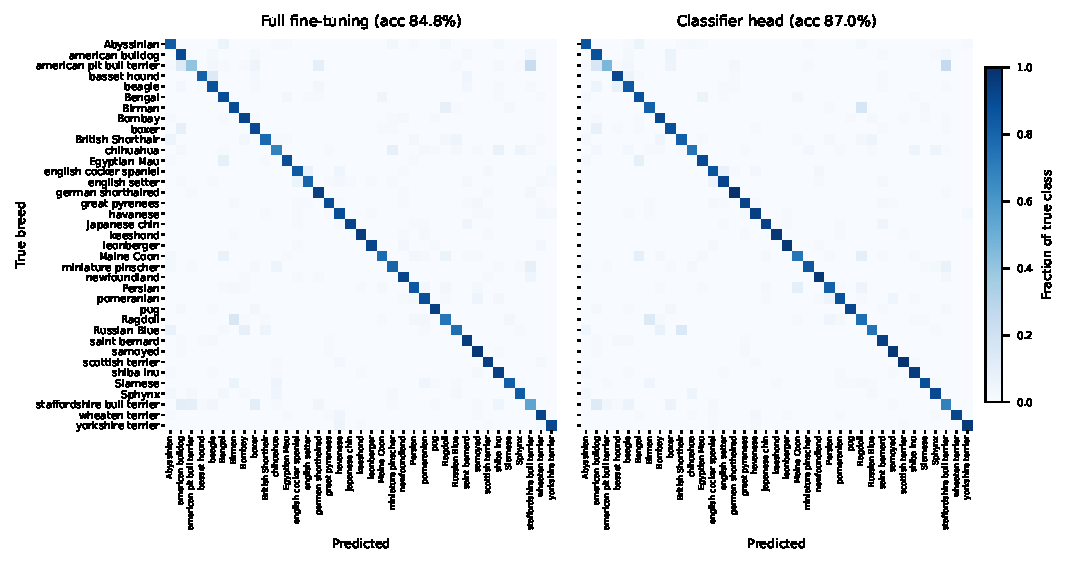
\includegraphics[width=\textwidth]{confusion_pair.pdf}
\caption{Row-normalised confusion matrices on the test set (rows: true breed, columns:
predicted breed). Full fine-tuning (left) and classifier-head training (right) share the
same class order. Full-size versions for all approaches, including logistic regression,
are in \texttt{results/figures/}.}
\label{fig:confusion}
\end{figure}

\paragraph{Confusion structure.}
Errors are concentrated among visually similar breeds. The most frequent confusion for
the best model (head-only) is \topPairA{} predicted as \topPairB{}
(\topPairCount{} images, \topPairFrac\% of that class); Table~\ref{tab:confusions} lists
the ten largest off-diagonal entries. Cat breeds with similar coat patterns
(e.g.\ Birman and Ragdoll, British Shorthair and Russian Blue, Persian and Maine Coon)
and the bull terrier breeds are repeatedly confused, while very distinctive breeds are
rarely wrong. The weakest breed by F1 is \worstClass{} (F1 \worstFone\%), the strongest
is \bestClass{} (F1 \bestFone\%). Figure~\ref{fig:examples} shows the most confident
correct and incorrect predictions of the classifier-head model; the failures typically
involve unusual poses, heavy occlusion, or a background that dominates the frame.

\begin{table}[t]
\centering
\caption{Largest off-diagonal entries of the classifier-head confusion matrix (best model).}
\label{tab:confusions}
\small
\begin{tabular}{llrr}
\toprule
True breed & Predicted as & Count & \% of true class \\
\midrule
american pit bull terrier & staffordshire bull terrier & 25 & 25.0 \\
Birman & Ragdoll & 16 & 16.0 \\
american pit bull terrier & american bulldog & 15 & 15.0 \\
Russian Blue & British Shorthair & 14 & 14.0 \\
Ragdoll & Birman & 13 & 13.0 \\
staffordshire bull terrier & american bulldog & 11 & 12.4 \\
Persian & Maine Coon & 9 & 9.0 \\
Maine Coon & Ragdoll & 9 & 9.0 \\
Maine Coon & Bengal & 9 & 9.0 \\
Egyptian Mau & Bengal & 8 & 8.2 \\
\bottomrule
\end{tabular}
\end{table}

\begin{figure}[t]
\centering
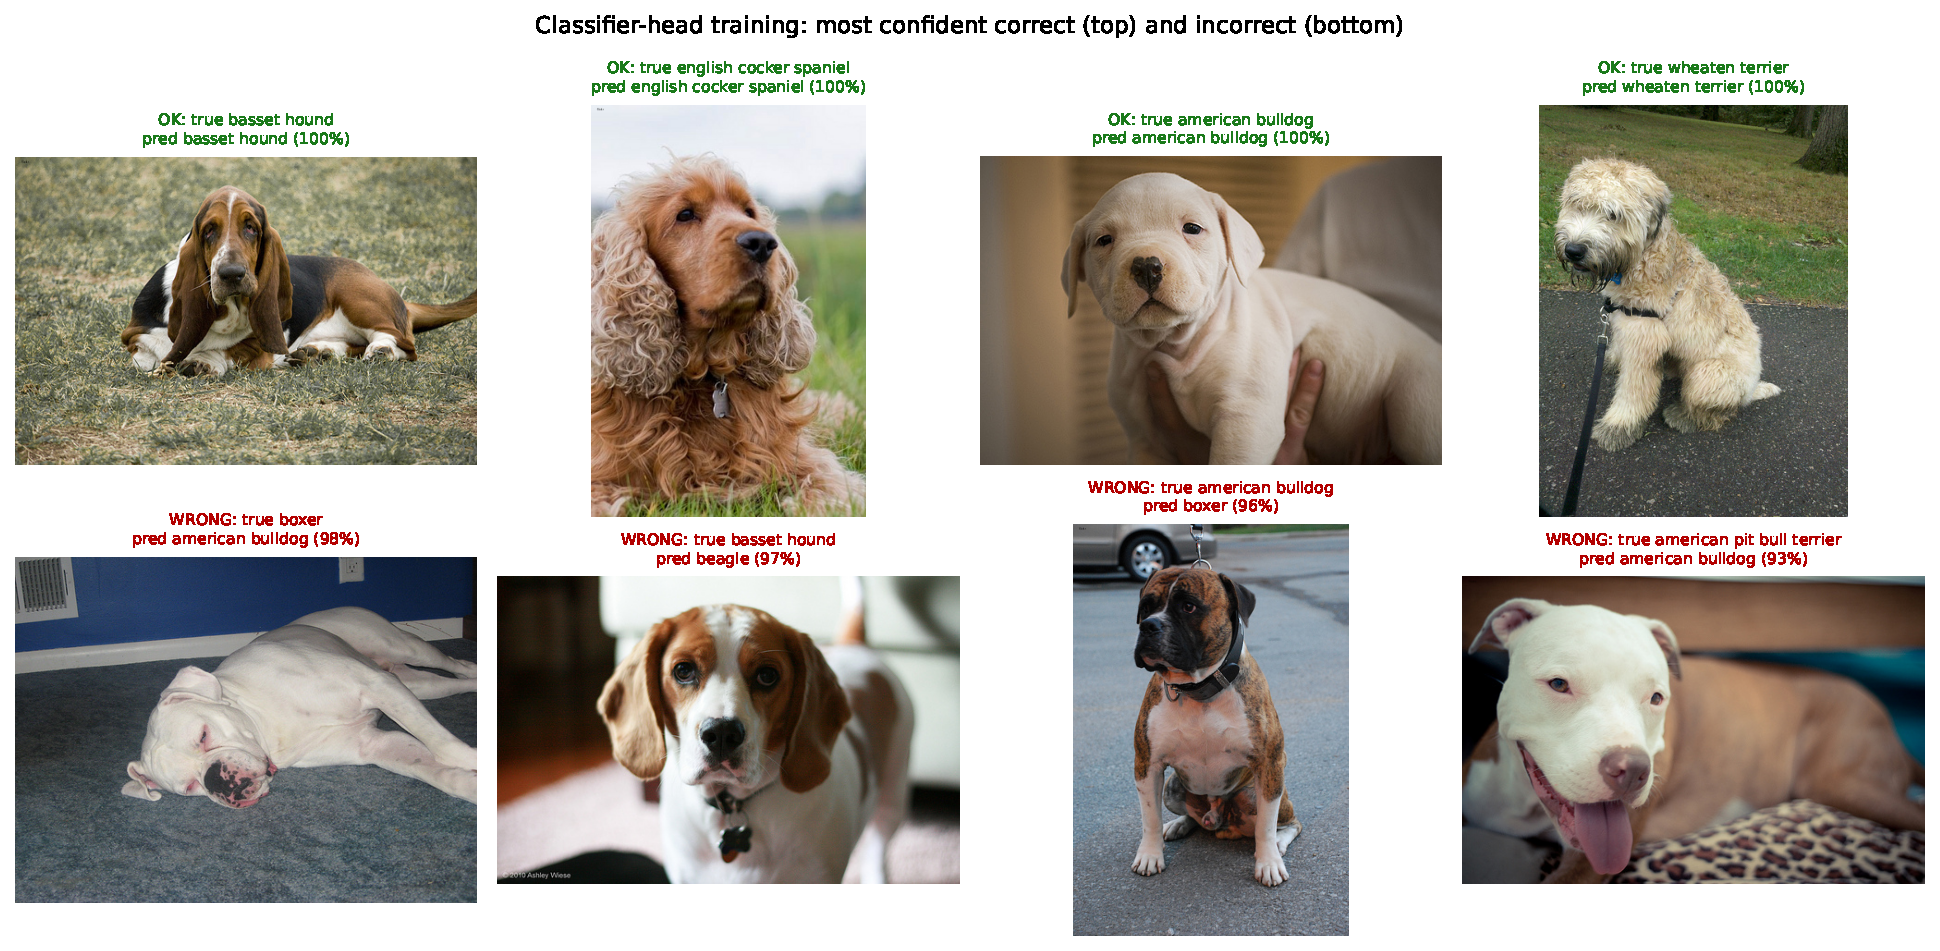
\includegraphics[width=\textwidth]{examples_head.pdf}
\caption{Most confident correct (top row) and incorrect (bottom row) test predictions of
the classifier-head model, with predicted confidence.}
\label{fig:examples}
\end{figure}

\section{Discussion}
\paragraph{Accuracy versus cost.}
Head-only training dominates the trade-off in this study: it is the most accurate method
(\headAcc\%) and costs \headTime{} minutes with \headParams{} parameters, against
\fullTime{} minutes and \fullParams{} parameters for full fine-tuning. Full fine-tuning
is \timeRatioFH$\times$ more expensive and \fullHeadDiff{} points less accurate, a
difference that is significant ($p\pFullHead$). The frozen-feature linear classifier is
by far the cheapest option (\lrTime{} minutes, compared with \fullTime{} for full
fine-tuning) and only \headLrDiff{} points behind the best model, so it is the rational
choice when compute is the binding constraint. The non-linear head is nevertheless worth
its extra parameters over the linear model ($p\pHeadLr$). The cost and accuracy
orderings therefore disagree: the cheapest neural strategy wins, and the most expensive
one does not.

\paragraph{Overfitting and generalization.}
Every method fits the training set almost perfectly, but the gaps differ. Full
fine-tuning reaches \fullTrainAcc\% training accuracy (gap \fullGap{}~pp), head-only
training \headTrainAcc\% (gap \headGap{}~pp), and logistic regression \lrTrainAcc\%
(gap \lrGap{}~pp); the 500-tree random forest memorizes the training set completely. The
head fits the training set even more closely than full fine-tuning yet generalizes
better, which locates the problem in the adaptable filters rather than in the classifier:
frozen ImageNet features stay fixed at test time, so the head can memorize without
changing the representation, whereas full fine-tuning can and does adapt filters to
training-specific cues. The gap alone still does not rank the methods, so we select by
validation macro-F1 and compare on test with paired tests.

\paragraph{Errors and limitations.}
The confusion analysis points to genuine fine-grained ambiguity rather than random
failure. Many errors are between breeds that differ mainly in ear shape, muzzle length, or
coat colour, and some images contain multiple animals or a small subject in a large
scene. The model sees a centre crop and no segmentation mask, so background context can
dominate. The 224-pixel input also discards fine texture that might separate, for
example, terrier varieties. A segmentation-aware crop (the dataset provides trimaps and
head boxes) or a higher input resolution would likely help, at additional cost.

Our study has several limitations. We use a single random seed and a single
train/validation split, so we cannot capture retraining variability: the paired McNemar
test quantifies test-set noise on fixed predictions, not variation across runs. The test
set is large (3,669 images), which keeps the binomial standard error around 0.7 points.
All neural training was done on a 4-core CPU with bfloat16 autocast, which is
reproducible but slow and may slightly change results relative to full-precision GPU
training. We compare one backbone and one set of hyper-parameters per strategy; a
learning-rate sweep for full fine-tuning could change the ranking. Finally, the dataset's license restricts use to
research, and the images are web-collected, so label noise and duplicate near-images
cannot be excluded.

\section{Reproducibility}
The code, split manifests, saved metrics, checkpoints, and figure-generation scripts are
publicly available at \url{https://github.com/Shihab7u/oxford-pet-transfer}. The
repository also contains the per-image test predictions and the scripts that generate
every table and figure. The environment is Python 3.13.9, PyTorch 2.15.0+cpu, TorchVision 0.29.2,
scikit-learn 1.9.1, SciPy 1.18.1, NumPy 2.5.4, pandas 3.1.1, and Matplotlib 3.11.2. The README gives
the download instructions and the exact commands for all three approaches. Seeds for
Python, NumPy, and PyTorch are fixed at 42, the split is persisted rather than
recomputed, and deterministic algorithms are requested (with \texttt{warn\_only} because
a few CPU kernels lack deterministic implementations). Remaining variation comes from
thread scheduling, bfloat16 arithmetic, and library versions.

\begin{thebibliography}{9}
\bibitem{parkhi2012cats}
O.~M. Parkhi, A.~Vedaldi, A.~Zisserman, and C.~V. Jawahar.
\newblock Cats and Dogs.
\newblock In \emph{IEEE Conference on Computer Vision and Pattern Recognition (CVPR)},
2012.

\bibitem{howard2019mobilenetv3}
A.~Howard, M.~Sandler, G.~Chu, L.-C. Chen, B.~Chen, M.~Tan, W.~Wang, Y.~Zhu,
R.~Pang, V.~Vasudevan, Q.~V. Le, and H.~Adam.
\newblock Searching for MobileNetV3.
\newblock In \emph{Proceedings of the IEEE/CVF International Conference on Computer
Vision (ICCV)}, 2019.

\bibitem{pedregosa2011sklearn}
F.~Pedregosa et al.
\newblock Scikit-learn: Machine Learning in Python.
\newblock \emph{Journal of Machine Learning Research}, 12:2825--2830, 2011.

\bibitem{paszke2019pytorch}
A.~Paszke et al.
\newblock PyTorch: An Imperative Style, High-Performance Deep Learning Library.
\newblock In \emph{Advances in Neural Information Processing Systems (NeurIPS)}, 2019.
\end{thebibliography}

\end{document}
